\documentclass[../competing_bandits.tex]{subfiles}
\begin{document}

\section{Algorithms' Performance in Isolation: Revisited}\label{section:revisited}

A natural question to ask is why we had to introduce the relative reputation proportion instead of simply using the mean to understand the results. For instance, the following would have been a natural conjecture:
\begin{conjecture}\label{conj:mean-trajectories}
\begin{enumerate}
\item To understand which algorithm would win in the competition game we could compare the mean reputation score of the two algorithms at $T_0$.\swcomment{should leave a pointer to the trajectories plot}
\item Given a sufficiently large $T_0$, if one algorithm's mean reputation trajectory lies above another, then the first algorithm prevails in the competition game.
\end{enumerate}
\end{conjecture}
\swcomment{why enumerate? sounds like two conjectures, but they are not. first part seems redundant}

However, we find a more nuanced picture. 

\begin{finding}
\textit{
Conjecture~\ref{conj:mean-trajectories} is false. Mean reputation trajectories do not suffice to explain the outcomes under competition. We observe in Figure \ref{sim_ht} that $\DG$ attains a larger market share than $\DEG$ even for large warm starts.\footnote{In the appendix we show that this holds for $K = 3$ and longer time horizons than we consider here as well.}}
\end{finding}

\begin{figure}[ht]
\caption{Distribution of reputation scores for Needle-in-Haystack at $t=500$ (smoothed using a kernel density estimate)}
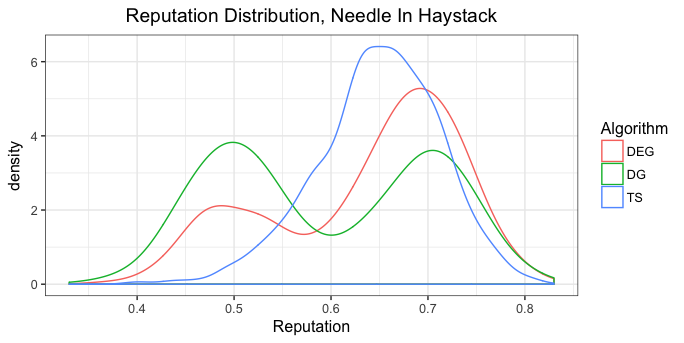
\includegraphics[scale=0.35]{figures/rep_distribution_nih}
\label{rep_dist_nih}
%\caption*{\tiny{The plots contain a kernel density estimate of the reputation distribution at $t = 500$}}
\end{figure}

\begin{figure}[ht]
\caption{Distribution of reputation difference $\TS-\DG$ for the Needle-in-Haystack (smoothed via a kernel density estimate)}
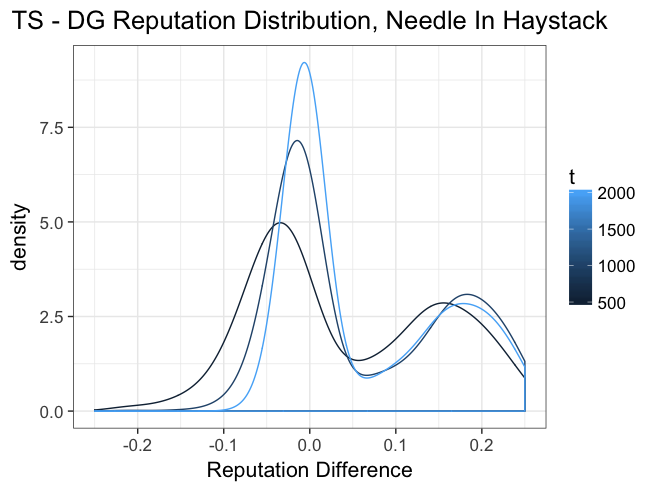
\includegraphics[scale=0.35]{figures/ts_dg_rep_diff_nih}
\label{ts_dg_rep_diff_nih}
%\caption*{\tiny{The plots contain a kernel density estimate of the difference in reputation between $\TS$ and $\DG$ across $t$}}
\end{figure}

To see what could go wrong, consider how an algorithm's reputation score is distributed at a particular time. That is, consider the empirical distribution of this score over different \MRVs.\swcomment{not sure what this means. over the randomness of \MRVs only? you mean marginal distribution?} For concreteness, we consider the needle-in-haystack instance at time $t=500$ (Figure \ref{rep_dist_nih}) since the intuition as to why the mean may be misleading is clearest on this instance (though the same result holds across the instances).

We see that the ``naive" algorithms $\DG$ and $\DEG$ have a bi-modal reputation distribution, whereas $\TS$ does not. The reason is that for this MAB instance,\swcomment{what is ``this''?} $\DG$ either finds the best arm and sticks to it, or gets stuck on the bad arms. This leads to two cases: $\DG$ either does slightly better than $\TS$ or where $\TS$ does substantially better than $\DG$.

However, the mean reputation trajectory \swedit{may fail to capture} this complexity since it simply takes average over different realizations of \MRVs. This may be inadequate for explaining the outcome of the duopoly game, given that the latter is determined by a simple comparison between the firm's reputation scores. Further, consider the difference in reputation scores (\emph{reputation difference}) between \TS and \DG on a particular \MRV. Let's plot the empirical distribution of the reputation difference (over the \MRVs) at a particular time point. Figure~\ref{ts_dg_rep_diff_nih} shows such plots for several time points.
\swcomment{I don't quite understand Figure~\ref{ts_dg_rep_diff_nih}. there are three curves, so I assume two black ones are for the two algos? If so, could you explain}
We observe that the distribution is skewed to the right, precisely due to the fact that $\DG$ either does slightly better than $\TS$ or does substantially worse. This means that the mean is not a good measure of the central tendency, or typical value, of the reputation difference distribution and overstates how well an advanced exploration algorithm (that will eventually find the best arm) should do in competition compared to a naive algorithm that may never find the best arm.


\end{document} 
%%% Local Variables:
%%% mode: latex
%%% TeX-master: "../competing_bandits"
%%% End:
